\documentclass{article}

\usepackage{tikz}
\usepackage{pgfplots}

\begin{document}

\pgfplotsset{
	small,
	title=Trimmed bounding boxes
}
\begin{center}
\begin{tabular}{rl}
	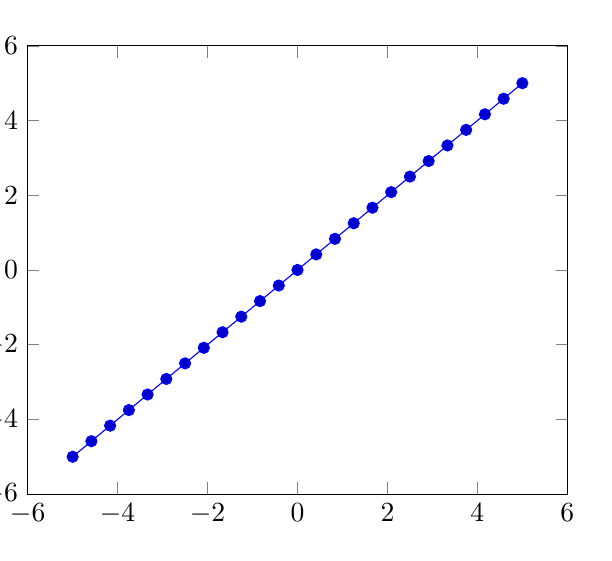
\begin{tikzpicture}[baseline,trim axis left]
		\begin{axis}
			\addplot {x};
		\end{axis}
	\end{tikzpicture}
	&
	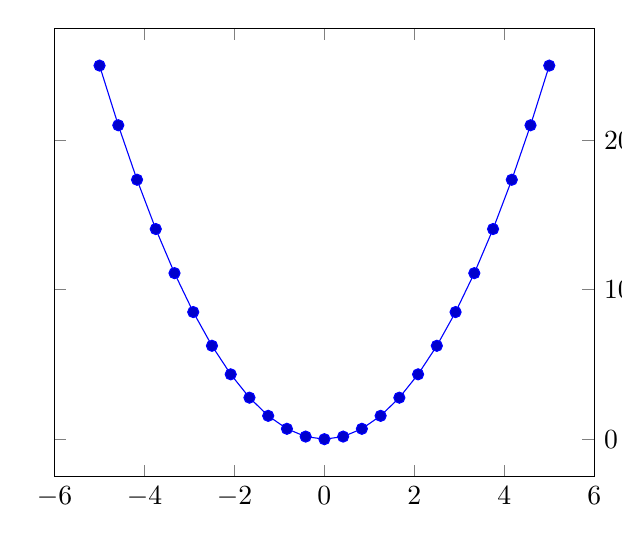
\begin{tikzpicture}[baseline,trim axis right]
	\begin{axis}[
		ylabel={$f(x)=x^2$},
		yticklabel pos=right,
		ylabel style={font=\Huge}]
		\addplot {x^2};
	\end{axis}
	\end{tikzpicture}
	\\
	%
	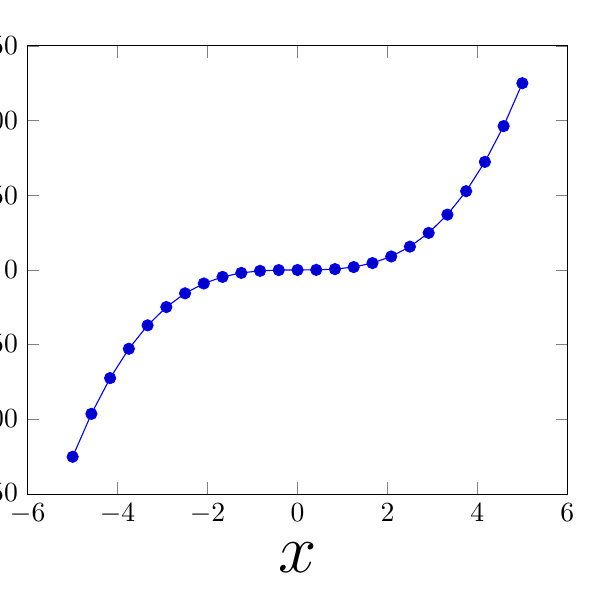
\begin{tikzpicture}[baseline,trim axis left]
	\begin{axis}[xlabel=$x$,xlabel style={font=\Huge}]
		\addplot {x^3};
	\end{axis}
	\end{tikzpicture}%
	&
	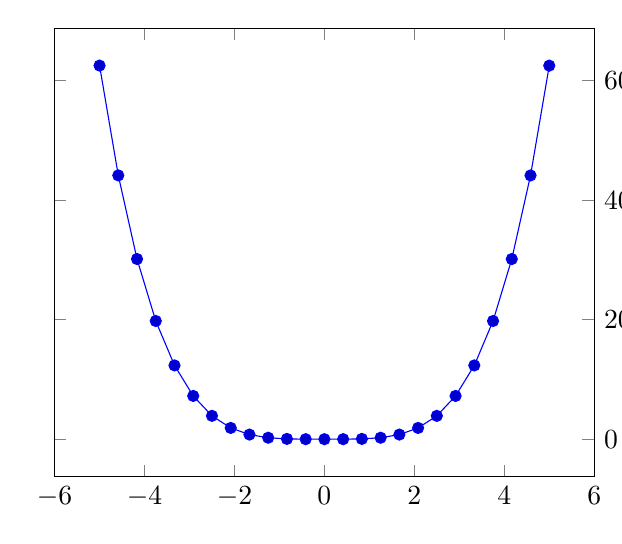
\begin{tikzpicture}[baseline,trim axis right]
	\begin{axis}[yticklabel pos=right]
		\addplot {x^4};
	\end{axis}
	\end{tikzpicture}%
	\\
\end{tabular}%
\end{center}

\end{document}
